%% cladograms.tex
%% Author: Leighton Pritchard
%% Copyright: James Hutton Institute
%% Introductory slides: Cladograms.

%
\begin{frame}
  \frametitle{Types of comparison}
    \begin{columns}[T] 
      \column{.5\textwidth} 
        \textcolor{RawSienna}{\textbf{Within species}}
        \begin{itemize}
	  \item e.g. between isolates/individuals (or between tissues$\ldots$)
	  \item \textcolor{hutton_green}{Which genome features may account for unique characteristics of organisms or cell-types (e.g. tumours)?}
	  \item \textcolor{hutton_blue}{what epigenetic changes occur in an individual?}
	\end{itemize}
      \column{.5\textwidth}
        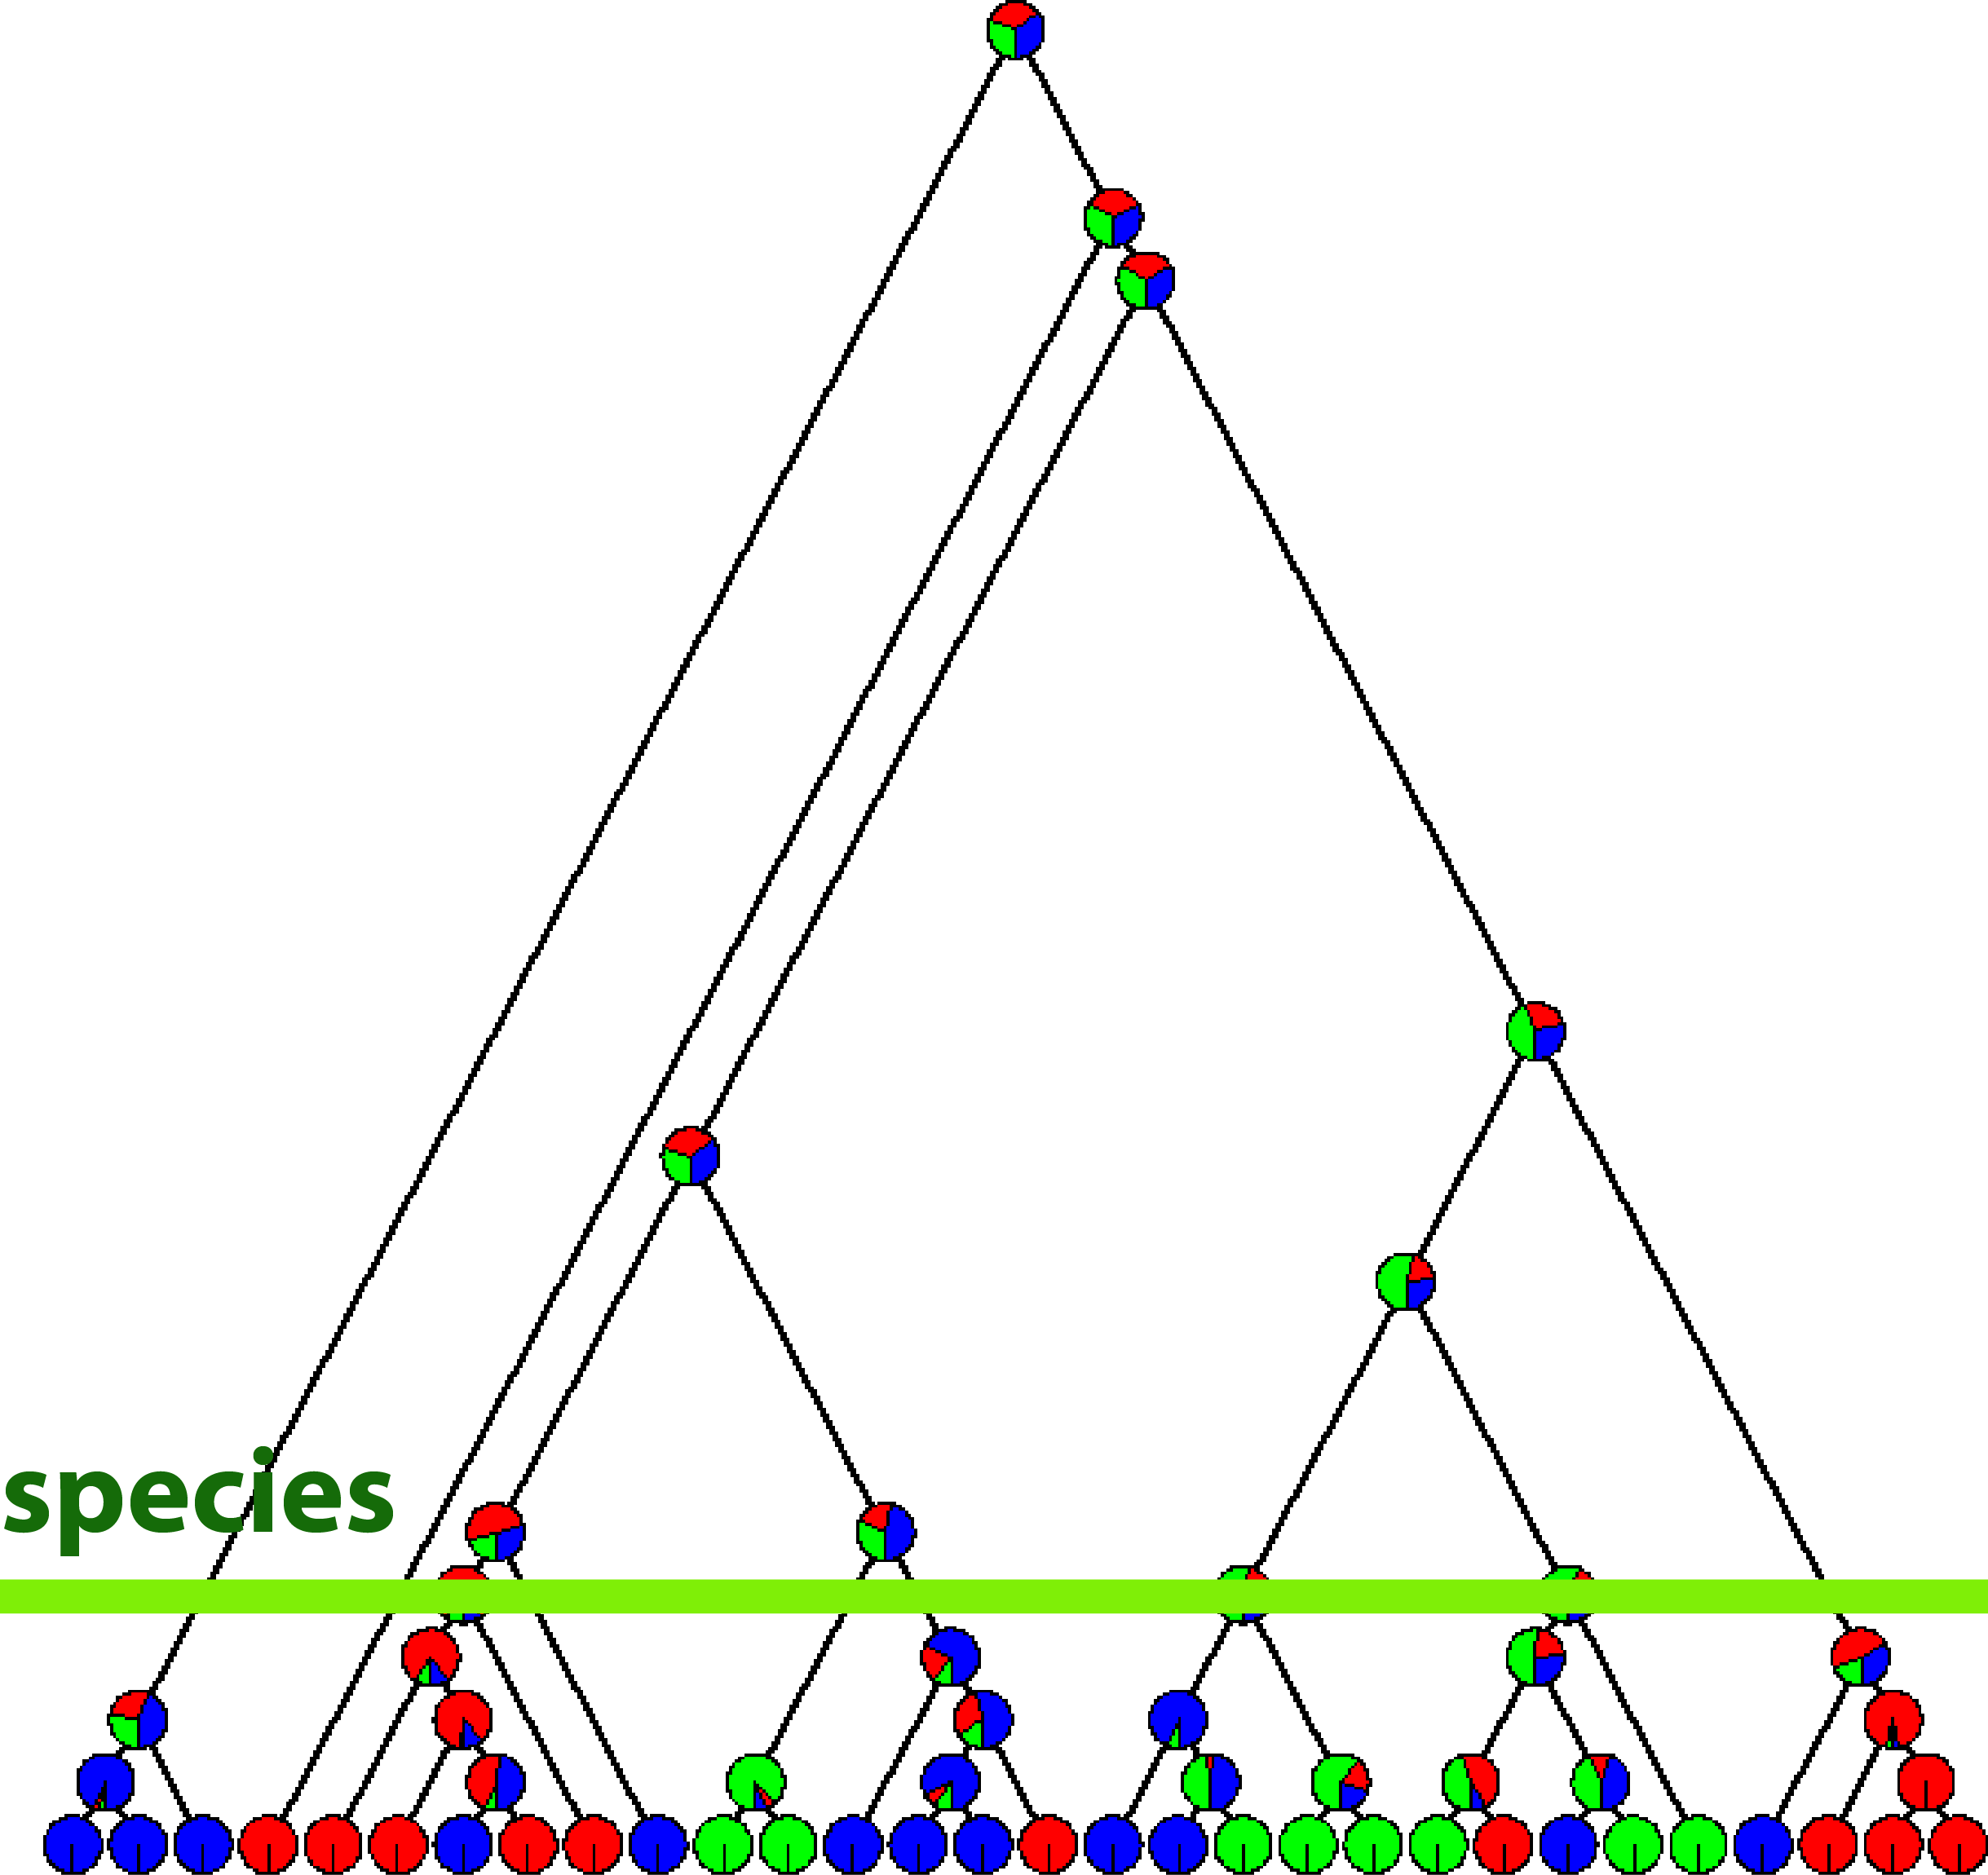
\includegraphics[width=\textwidth]{images/cladogram_species}
    \end{columns}  
\end{frame}

%
\begin{frame}
  \frametitle{Types of comparison}
    \begin{columns}[T] 
      \column{.5\textwidth} 
        \textcolor{RawSienna}{\textbf{Within genera/between species}}
        \begin{itemize}
	  \item comparison between groups of individuals
	  \item \textcolor{hutton_green}{what genome features show evidence of selective pressure?}
	  \item \textcolor{hutton_blue}{which features/changes are associated with species phenotype/adaptation?}      
        \end{itemize}
      \column{.5\textwidth}
        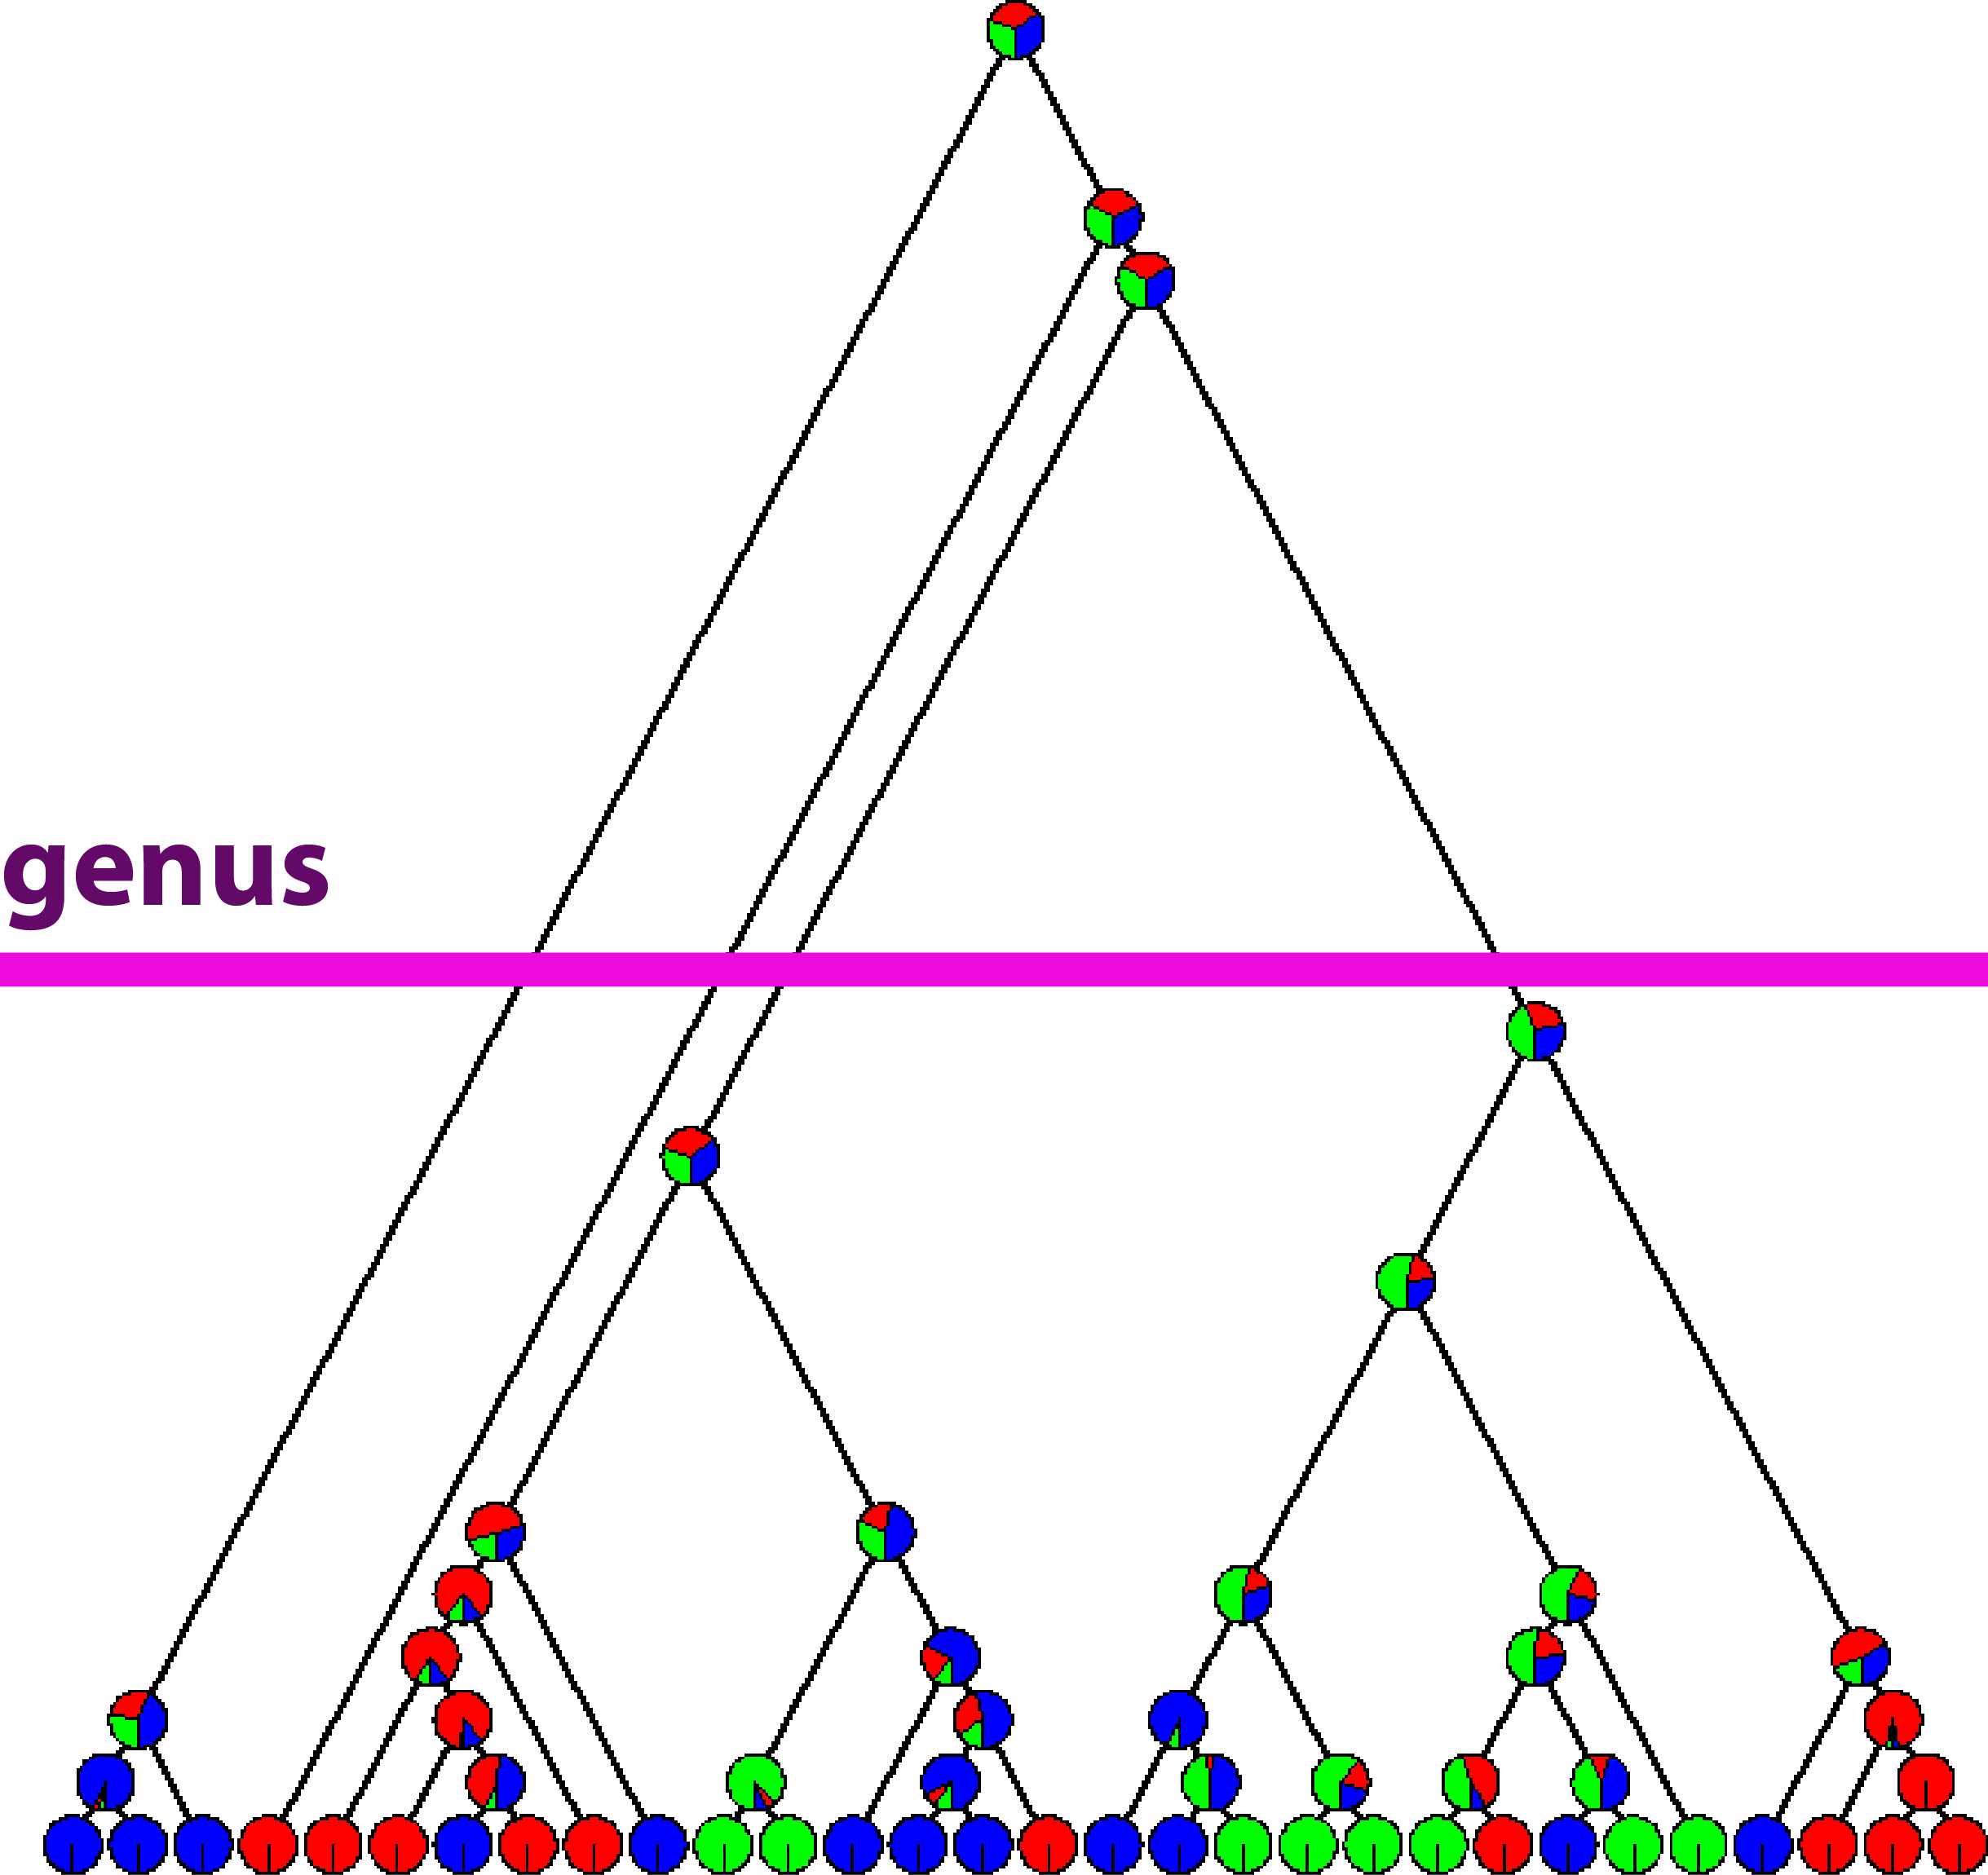
\includegraphics[width=\textwidth]{images/cladogram_genus}
    \end{columns}  
\end{frame}

%
\begin{frame}
  \frametitle{Types of comparison}
    \begin{columns}[T] 
      \column{.5\textwidth} 
        \textcolor{RawSienna}{\textbf{Between subgroups}}
        \begin{itemize}
          \item e.g. comparisons across many diverse individuals
          \item \textcolor{hutton_green}{what are the \textit{core set} of genome features that define a subgroup or genus?}
          \item \textcolor{hutton_blue}{what functions are present/absent between groups?}
        \end{itemize}
      \column{.5\textwidth}
        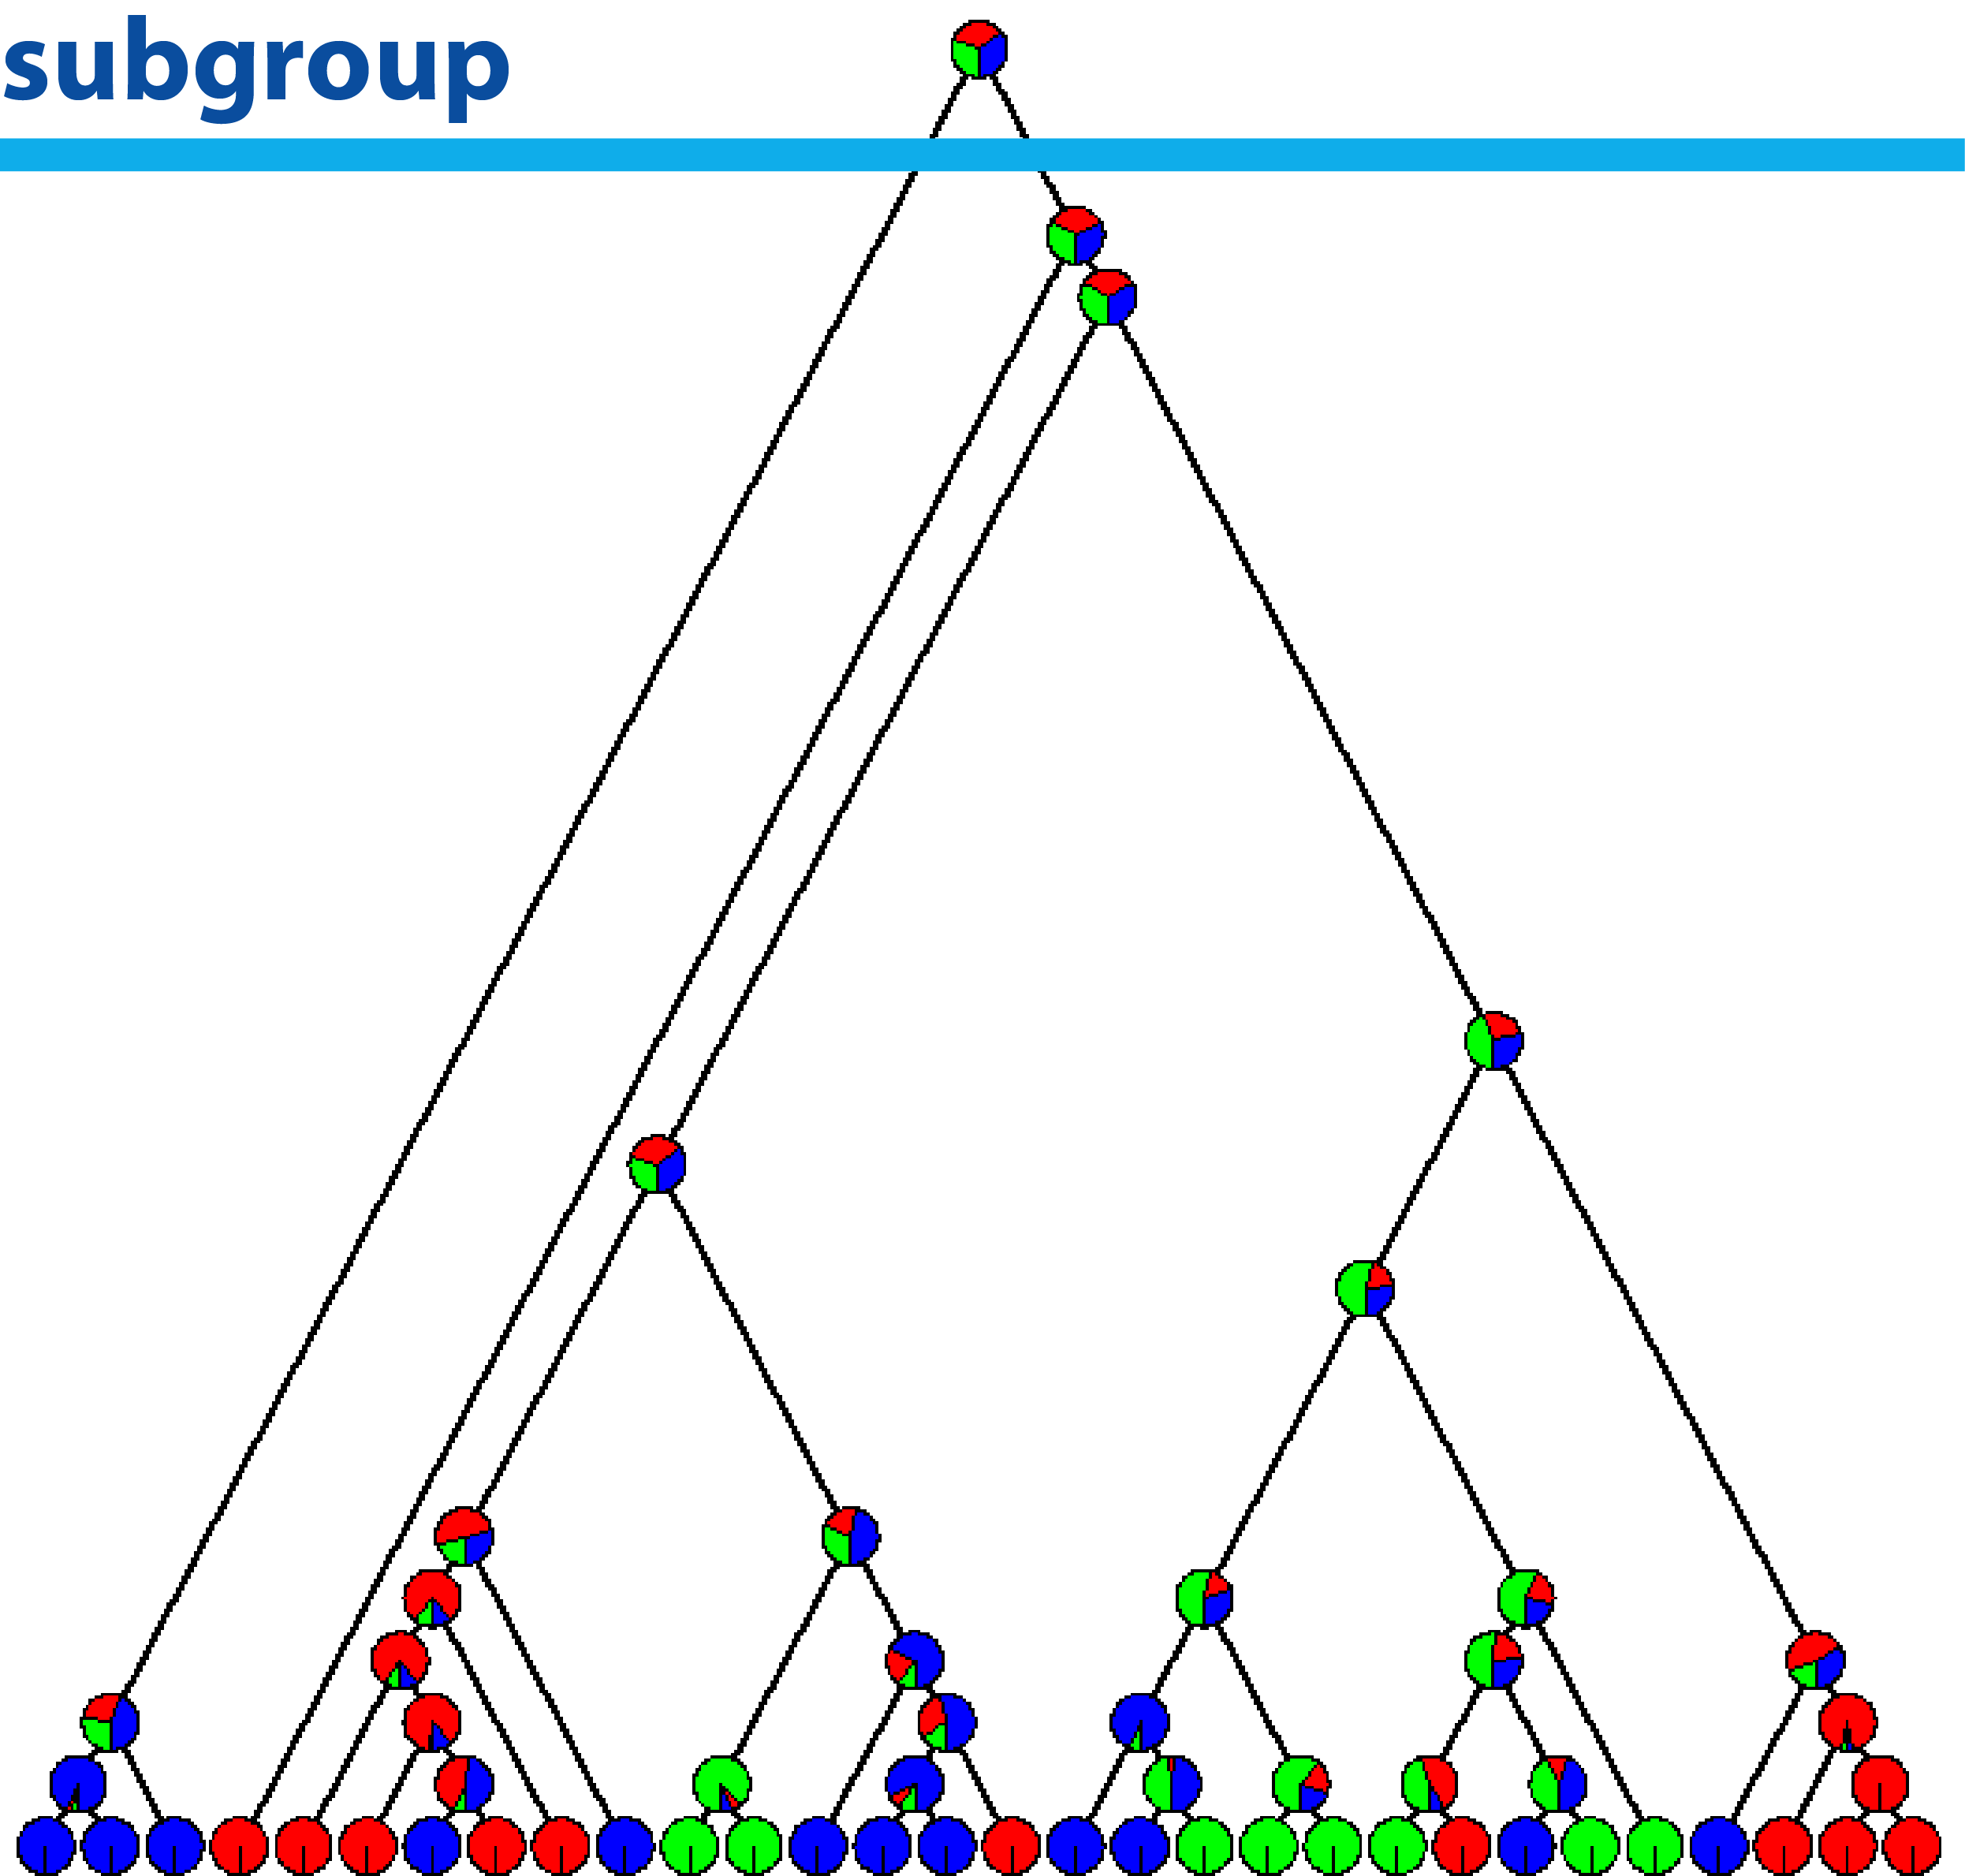
\includegraphics[width=\textwidth]{images/cladogram_subgroup}
    \end{columns}  
\end{frame}